\chapter{Introduction}\label{chap:theory}
\minitoc
\vfill
\mybox{
This chapter gives an introduction to the geological storage of carbon dioxide, geoelectrical monitoring, and the studied field site.
Finally, the research objectives and structure of this thesis are outlined.
The given introduction aims to provide a basis for the individual papers comprised in this cumulative thesis and does not attempt to represent a general overview.
}

\section{Geological \co storage}

\subsection{Motivation and potential}
\citep{Archie1942} 
\Blindtext



\begin{figure}[htbp]
\centering
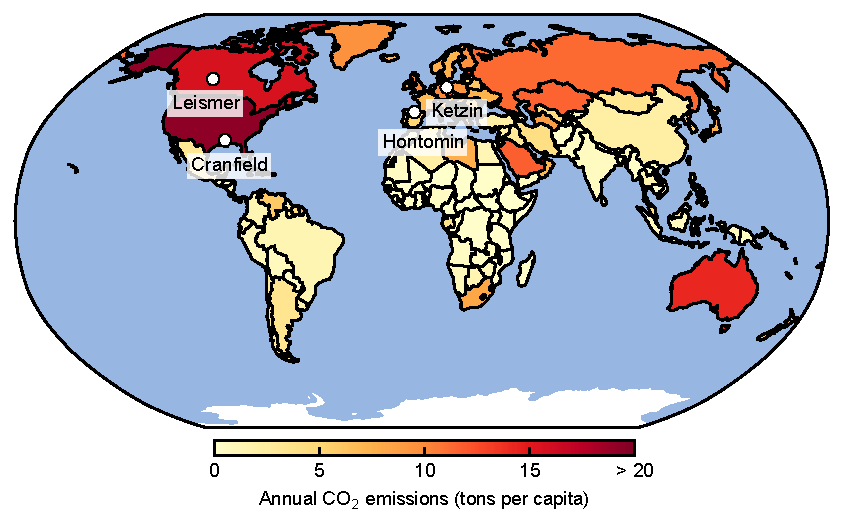
\includegraphics[width=.9\textwidth]{figs/map.pdf}
\caption{Overview of deep permanent electrode installations. The map is colored by annual \co emissions in metric tons per capita averaged between 1960 and 2015 \citep{Bank2015}.}
\label{fig:map}
\end{figure}
%

\cref{chap:theory} introduces the underlying inversion theory as used in the code by \cite{Ruecker2017}.
